\chapter{Motivación y Métodos Numéricos}\label{cap1INTRO}


% --- Define análisis y análisis no lineal ---
El análisis de una estructura consiste en establecer ciertas hipótesis mecánicas y físicas sobre el comportamiento de la misma, obtener y resolver el modelo matemático correspondiente, e interpretar los resultados. %
%
Si las hipótesis establecidas son tales que las ecuaciones del modelo matemático son no lineales, el análisis es considerado no lineal. %
%
La validez de los resultados de un análisis estructural depende de las aproximaciones de la realidad dadas por las hipótesis definidas y de la precisión de la resolución del modelo matemático correspondiente. %
% --------------------------

%
Dado este marco, se enumeran a modo de motivación una serie de estructuras o problemas estructurales reales que requieren el uso de modelos no lineales. %
%
Posteriormente, se introducen algunos métodos numéricos que permiten, mediante herramientas computacionales, llevar a cabo el análisis no lineal de una estructura.


\section{Motivación y enfoque}

\subsection*{Motivación}

El análisis no lineal de estructuras forma parte esencial de los conocimientos de los ingenieros estructurales en  disciplinas como: Civil (infraestructura), Mecánica, Naval, Aeroespacial, Automotriz, Biomecánica, etc.  

En algunas aplicaciones en el área Civil, en particular en estructuras de edificación sencillas, los efectos resultantes del comportamiento no lineal de las estructuras están contemplados mediante procedimientos codificados en las normas de diseño estructural (ver por ejemplo ACI 318-14, AISC 360-16, Eurocódigos).

No obstante, para estructuras que se apartan de las hipótesis asumidas en los procedimientos codificados, las normas mencionadas describen y admiten análisis más refinados de los efectos resultantes de la respuesta no lineal de las estructuras. %
%
La necesidad de llevar adelante estos análisis se vuelve imprescindible para ciertos tipos de estructuras que trabajan en régimen no lineal bajo cargas de servicio. Algunos ejemplos de estas estructuras son:


\begin{itemize}
	\item mástiles atirantados \citep{Sparling1995},
	\item puentes suspendidos \citep{Larsen2000},
	\item puentes atirantados \citep{Wu2015,Madrazo-Aguirre2015},
	\item análisis de placas o cáscaras delgadas \citep{Hunt1998},
	\item estructuras reticuladas y aporticadas esbeltas \citep{Morozov2011},
	\item cubiertas con membranas tensas \citep{Bridgens2012},
	\item cubiertas formadas por cables \citep{Feng2013}.
\end{itemize}

Adicionalmente, las normas modernas de diseño estructural admiten la determinación de la capacidad de las estructuras o componentes estructurales mediante análisis numéricos apropiados. A modo de ejemplo, la norma EN 1993-1-6 aplicable a cáscaras de acero propone una secuencia progresiva de análisis de distinta complejidad de manera de llegar a determinar la capacidad de una cáscara de acero. Dicha secuencia de análisis es resumida a continuación:
%
\begin{enumerate}
	\item[1)]Análisis Elástico Lineal (LA),
	\item[2)]Análisis de Bifurcación Elástico Lineal (LBA),
	\item[3)]Análisis No Lineal Geométrico Elástico (GNA),
	\item[4)]Análisis No Lineal Material (MNA),
	\item[5)]Análisis No Lineal Geométrico Elástico con Imperfecciones (GNIA),
	\item[6)]Análisis No Lineal Material y Geométrico con Imperfecciones (GMNIA).
\end{enumerate}

En la Figura~\ref{fig:fig0} se presentan de forma esquemática las curvas de carga-deformación resultantes de los análisis enumerados anteriormente. %
%

\begin{figure}[htb]
	\centering
   \def\svgwidth{0.75\textwidth}
   \input{../fig/Fig0_modif.pdf_tex}
	\caption{Curvas de carga-desplazamiento esquemáticas para distintos análisis.}
	\label{fig:fig0}
\end{figure}

La norma recomienda realizar los distintos análisis utilizando el Método de los Elementos Finitos (MEF), el cual será presentado en la Sección \ref{FEM}. %
%
Al usar modelos numéricos para realizar la secuencia de análisis descritos se debe comenzar por el análisis más sencillo (LA) e incorporar gradualmente complejidades de análisis y examinando mediante un análisis crítico los resultados que se van obteniendo. %
%
Comenzar los análisis partiendo de un modelo complejo puede ser peligroso ya que no se tendrá una idea clara de qué resultados se deben esperar y sobre dónde podrían haber errores ocultos en el modelo o la solución numérica.

La capacidad de realizar análisis no lineales es crítica también al diseñar estructuras sometidas a acciones accidentales como por ejemplo impacto o explosión. Al realizar el diseño de estructuras bajo hipótesis de colapso progresivo, como puede ser la eliminación de una columna en un edificio, se debe considerar que la estructura experimenta grandes deformaciones y el equilibrio en esas situaciones debe necesariamente contemplar efectos no lineales tanto en la geometría como en los materiales.

\subsection*{Enfoque}

En este documento se aborda el análisis no lineal de estructuras discretas, es decir que no se presentan métodos para análisis no lineal de sólidos continuos arbitrarios. %
%
En particular, se consideran estructuras formadas mediante barras articuladas (reticulados) sometidas a distintas condiciones de apoyo y esfuerzos en las articulaciones o nodos. %
% ------------------------------



La consideración de estructuras reticuladas permitirá presentar conceptos y formulaciones de complejidad relativamente baja sin dejar de lado los conceptos centrales referentes a modelos estructurales no lineales. 

Estos elementos estructurales relativamente sencillos permitirán idealizar otros tipos de estructuras, como pórticos o arcos, mediante estructuras reticuladas equivalentes. %
%
Esto permitirá observar fenómenos como flexión en componentes estructurales y en estructuras completas sin necesidad de desarrollar formulaciones de elementos de tipo viga. %
% -------------------------------------------

En el contexto de estructuras de barras, se introducen los conceptos de no linealidad geométrica, inestabilidad, no linealidad material y dinámica no lineal. %
%
Cabe aclarar que no se cubrirán todas las posibles fuentes de no linealidad en el comportamiento de estructuras, en particular no se estudiarán problemas de contacto entre componentes estructurales, ni cargas dependientes de la geometría de la estructura (\textit{following loads}).

\section{Métodos Numéricos para Ecuaciones No Lineales} \label{sec:mnecnl}

Determinar las configuraciones de equilibrio de una estructura con comportamiento no lineal requiere la capacidad de resolver sistemas de ecuaciones no lineales. Por ende, los procedimientos de análisis no lineal de estructuras están directamente basados en métodos numéricos de resolución de sistemas de ecuaciones no lineales. %
%
En varios casos, las aplicaciones prácticas de resolución de estructuras han sido las precursoras de los que posteriormente serían métodos numéricos aplicados a diversas ramas de la Ingeniería, como el Método de los Elementos Finitos \citep{Zienkiewicz1972} (ver  \citep{crisfield1996non,Bathe2014} por más detalle).
% ---------------------------------------------------------------

Con el objetivo de evitar la asimilación en simultáneo de procedimientos numéricos y conceptos estructurales, se opta por comenzar presentando de forma aislada los métodos numéricos más importantes para, en capítulos posteriores, aplicarlos en el contexto de problemas estructurales. 

El estudio y desarrollo de estos métodos numéricos forma parte del área llamada Continuación Numérica, perteneciente a la disciplina Matemática Aplicada \citep{Doedl2014Slides}. %
%
En las siguientes secciones se presentan las tres clases principales de métodos numéricos que son de utilidad para resolver sistemas de ecuaciones no lineales, descritos a continuación: %
%
%
\begin{itemize}
	\item Métodos Incrementales,
	\item Métodos Iterativos,
	\item Métodos de Longitud de Arco.
\end{itemize}

Actualmente existen diversos programas generales basados en implementaciones de estos métodos. %
%
Asimismo, estos programas pueden ser aplicados al estudio de problemas de estabilidad estructural, como se puede ver en trabajos como \citep{Wadee245}.

En este documento se utiliza la siguiente notación para representar vectores, matrices y escalares: letras minúsculas en negrita para vectores (ej. $\bfu$), letras mayúsculas en negrita para matrices (ej. $\bfK$) y letras mayúsculas o minúsculas para escalares (ej. $x$ o $E$).

Se considera una estructura discreta como aquella cuya geometría es determinada a partir de un número ($n\in\mathbb{N}$) de valores, o grados de libertad, dados por $\bfx\in \mathbb{R}^n$. %
%
La estructura es sometida a un conjunto de cargas externas y se define un parámetro real $\lambda\in \mathbb{R}^+$ que corresponde al factor de carga. %
%
Es decir, $\lambda$ es un parámetro que indica qué múltiplo de la carga externa definida está aplicada sobre la estructura. %
%
Se considera que $\lambda=0$ implica una estructura descargada y que eso corresponde a la estructura en la configuración sin deformaciones, o lo que es lo mismo $\bfx=0$.


En situaciones donde $\lambda>0$, las condiciones de equilibrio, compatibilidad y relación constitutiva del material proveen un sistema de ecuaciones no lineales que vinculan $\bfx$ con $\lambda$ mediante una función no lineal $\bfg:\mathbb{R}^n \times \mathbb{R}^+ \longrightarrow \mathbb{R}^n$ dada por:
%
\begin{equation}\label{ec1}
\bfg(\bfx,\lambda)=0.
\end{equation}

La ecuación anterior se puede reducir a un caso menos general asumiendo que las cargas son independientes de los desplazamientos. En ese caso, la no linealidad respecto de $\bfx$ estará contenida completamente en una función vectorial de fuerzas internas $\bff:\mathbb{R}^n \longrightarrow \mathbb{R}^n$ mientras que las cargas externas están dadas por un vector fijo $\bfv \in \mathbb{R}^n$. %
%
La ecuación resultante es:
%
\begin{equation}\label{ec2}
\bff(\bfx)-\lambda \bfv=0.
\end{equation}

Las soluciones de los sistemas (\ref{ec1}) o (\ref{ec2}) determinan el conjunto de todas las parejas de valores $(\lambda,\bfx)$ que satisfacen dichos sistemas no lineales. De forma equivalente, las soluciones se pueden considerar como trayectorias que pasan por $(0,0)$ en el espacio de configuraciones de la estructura $\mathcal{S} \equiv \mathbb{R}^+ \times \mathbb{R}^n$ y que satisfacen la Ecuación~\eqref{ec2} en todo punto de dichas trayectorias. Aquí y en los capítulos siguientes se llamará a dichas trayectorias como Curvas de Carga-Desplazamiento.

A continuación, se describen métodos para hallar soluciones numéricas de (\ref{ec1}) o en su defecto (\ref{ec2}).

\subsection{Métodos Incrementales}\label{Increm}

En esta familia de métodos, se transforma el problema de determinar las trayectorias dadas por puntos $P=(\lambda,\bfx)\in\mathcal{S}$ que verifican la Ecuación~\eqref{ec2}, en hallar la solución de una ecuación diferencial ordinaria (E.D.O).

Para ello se considera que las trayectorias se pueden parametrizar respecto de $\lambda$, con lo cual podemos escribir: $(\lambda,\bfx(\lambda))$. Estos puntos satisfacen la ecuación no lineal dada por la Ecuación~\eqref{ec2} para todo $\lambda$, por lo tanto:
%
\begin{equation}\label{ec3}
\bff(\bfx(\lambda))-\lambda \bfv=0.
\end{equation}

Derivando ambos miembros de la Ecuación~\eqref{ec3} respecto de $\lambda$ se obtiene:
%
\begin{equation}\label{ec4}
\bfF_x(\bfx(\lambda))\dot{\bfx}(\lambda)-\bfv=0,
\end{equation}
%
donde $\bfF_x$ es una matriz cuadrada (llamada matriz tangente) cuya entrada $ij$ está dada por $(\bfF_x)_{i,j}=\frac{\partial f_i}{\partial x_j}$. %
%
Asumiendo que $\bfF_x$ es invertible se obtiene la siguiente E.D.O. de primer orden:
%
\begin{equation}\label{ec5}
\dot{\bfx}(\lambda)=\bfF_x^{-1}(\bfx(\lambda))\bfv.
\end{equation}

La Ecuación~\eqref{ec5} en conjunto con la condición inicial $\bfx(0)=0$, determinan un Problema de Valores Iniciales dado por:
%
\begin{equation}\label{EDO}
\text{E.D.O}
	\begin{cases} 
		\dot{\bfx}(\lambda)=\bfF_x^{-1}(\bfx(\lambda))\bfv \\
		\bfx(0)=0
	\end{cases}
\end{equation}
%
Por conveniencia se hará referencia a este problema como una E.D.O. %

A partir de este punto se puede aplicar cualquier método numérico para la resolución de E.D.Os. %
%
Ver por ejemplo \citep{kahaner1989numerical}, \citep{butcher2004numerical} o las Notas de Teórico del curso \textit{Métodos Numéricos} (dictado por el Instituto de Matemáticas y Estadística de la Facultad de Ingeniería de la Universidad de la República).

A modo de ejemplo, se introduce un método extremadamente sencillo y suficientemente general como para poder apreciar este tipo de soluciones: el Método de Euler Hacia Adelante (en inglés: \textit{Forward Euler}).

\subsubsection{Método de Euler Hacia Adelante}\label{FEuler}

Dada una E.D.O. de primer orden genérica con variable independiente $t$, $\dot{\bfx}(t)=\bfh(\bfx(t),t)$ y una aproximación numérica aceptable de la solución de la E.D.O. en $t_k$, $\bfx_k\approx \bfx(t_k)$, se puede escribir el siguiente desarrollo de Taylor de $\bfx(t)$ en $t_k$ (con $\xi\in(t_k,t)$):
%
\begin{equation}\label{ec6}
\bfx(t)=\bfx(t_k) + \dot{\bfx}(t_k)(t-t_k) + \frac{1}{2}\ddot{\bfx}(\xi)(t-t_k)^2.
\end{equation}

Evaluando la expresión dada por la Ecuación~\eqref{ec6} en $t=t_k+\Delta t$ y usando que $\dot{\bfx}=\bfh(\bfx,t)$ se tiene:
%
\begin{equation}\label{ec7}
\bfx(t_k+\Delta t)=\bfx(t_k) + \bfh(\bfx(t_k),t_k)\Delta t + \frac{1}{2}\ddot{\bfx}(\xi)\Delta t^2.
\end{equation}

Despreciando el término de segundo orden y llamando $\bfx_{k+1}$ y $\bfx_k$ a las aproximaciones de $\bfx(t_k+\Delta t)$ y $\bfx(t_k)$ respectivamente, se obtiene:
%
\begin{equation}\label{ec8}
\textit{F.Euler}
	\begin{cases} 
	\bfx_{k+1}=\bfx_k + \Delta t\cdot \bfh(\bfx_k,t_k) \\
	\bfx_0=\bfx(0)
	\end{cases}
\end{equation}

El Método de Euler Hacia Adelante (\textit{Forward Euler}) queda definido mediante la expresión de la Ecuación~\eqref{ec8} y es un método explícito dado que solo utiliza valores ya calculados para determinar el próximo incremento. %
%
Existen otros métodos, implícitos, en los cuales el incremento está dado por la solución de una ecuación implícita (ver las referencias sobre métodos numéricos para resolución de E.D.Os citadas por más detalle).

Es claro a partir de la Ecuación~\eqref{ec7} que en cada paso este método se aleja de la solución exacta en un factor $O(\Delta t^2)$. Esto hace que este método, y todos los otros métodos incrementales también, sufran de un efecto de deriva, llamado \textit{drift}, de la solución numérica respecto de la solución exacta teórica.

Este \textit{drift} se puede reducir utilizando métodos de mayor orden, los cuales son más costosos del punto de vista computacional, o usando incrementos $\Delta t$ lo suficientemente pequeños como para alcanzar una precisión requerida en un cierto valor objetivo $t^*$.

Por último, es necesario comentar sobre el costo computacional del Método de Euler Hacia Adelante. %
%
A partir de la Ecuación~\eqref{ec8} se puede ver que cada paso del método implica una evaluación de la función $\bfh(\bfx,t)$. %
%
Generalmente, el costo de la evaluación de $\bfh(\bfx_k,t_k)$ supera con facilidad al resto de las operaciones de punto flotante necesarias para completar el paso incremental. %
%
En el caso específico de la resolución de una ecuación no lineal mediante un método incremental, dicha evaluación corresponde a $\bfh(\bfx_k,t_k)=\bfF_x^{-1}(\bfx_k)\bfv$, lo cual tiene el costo de evaluar $\bfF_x(\bfx_k)$ y luego resolver un sistema lineal ($\bfF_x(\bfx_k)\bfz=\bfv$) con costo de $O(n^3)$ operaciones en punto flotante en general (posiblemente menor si $\bfF_x$ es una matriz esparza).

\subsubsection{Ejemplo Numérico 1: Solución Incremental}\label{ej1}

A continuación se resuelve numéricamente la ecuación no lineal:
%
\begin{equation}\label{ec:ejemplo1}
x-\frac{3}{2}x^2+\frac{1}{2}x^3-\lambda=0.
\end{equation}

Esta ecuación está vinculada al análisis geométricamente no lineal de una estructura conocida como cercha de Von Mises, ver la Sección~\ref{MisesTruss}. La estructura tiene un solo grado de libertad de desplazamiento vertical del centro de la cercha y exhibe un comportamiento de tipo \textit{snap-through}, es decir que al alcanzar un cierto nivel de carga pierde estabilidad, produciéndose un ``salto'' a otra configuración de equilibrio.


Es claro que el problema de encontrar la carga ($\lambda$) que corresponde a un cierto desplazamiento ($x$) es trivial, solamente se debe despejar $\lambda$ de la Ecuación (\ref{ec:ejemplo1}) y evaluar dicha expresión en el valor de desplazamiento dado ($x$).

El problema inverso, en el cual dado el nivel de carga se quiere hallar el desplazamiento correspondiente de la estructura, requiere el uso de un método numérico para resolución de ecuaciones no lineales, como por ejemplo el procedimiento incremental visto anteriormente.

Dada la Ecuación~\eqref{ec:ejemplo1} y comparando con la Sección~\ref{Increm} se puede ver que $\bfv = 1$ y que las funciones $\bff$ y $\bfF_x$ quedan definidas como: 
%
\begin{equation}
	\bff(x)=x-\frac{3}{2}x^2+\frac{1}{2}x^3 \qquad \text{y} \qquad  \bfF_x(x)=1-3x+\frac{3}{2}x^2,
\end{equation}
respectivamente. %
%
Se desea obtener estimaciones de valores de la solución ($x_k$) en incrementos $\Delta \lambda=0.02$ hasta alcanzar un valor objetivo $\lambda^*$. %

El Método de Euler Hacia Adelante permite, comenzando desde $x_0=0$ y $\lambda_0=0$, hallar las soluciones ($x_1, x_2, ...$) de forma incremental mediante la expresión:
%
\begin{equation}
	x_{k+1} = x_k + 0.02 \left(\frac{1}{1-3x_k+\frac{3}{2}x_k^2}\right).
\end{equation}
%
El método es implementado a través del código de Octave mostrado al final de esta sección en el Código~\ref{cod:ejnonlin}.

En la Figura~\ref{fig:fig1} se muestran los resultados obtenidos al aplicar el método para diferentes valores de $\lambda$ objetivo. %
En la gráfica de la izquierda se puede ver el efecto de \textit{drift}, o separación, entre la solución exacta y la solución numérica incremental. %
En la gráfica de la derecha se muestra lo que ocurre cuando el método es aplicado para un valor $\lambda$ superior al correpsondiente a un punto con tangente horizontal (que llamaremos: Punto Límite). %
%
Se ve claramente que la solución numérica se aleja desproporcionadamente de la solución exacta.

\begin{figure}[htb]
	\centering
	\resizebox{\textwidth}{!}{% Title: gl2ps_renderer figure
% Creator: GL2PS 1.4.0, (C) 1999-2017 C. Geuzaine
% For: Octave
% CreationDate: Fri Dec 29 11:28:13 2017
\setlength{\unitlength}{1pt}
\begin{picture}(0,0)
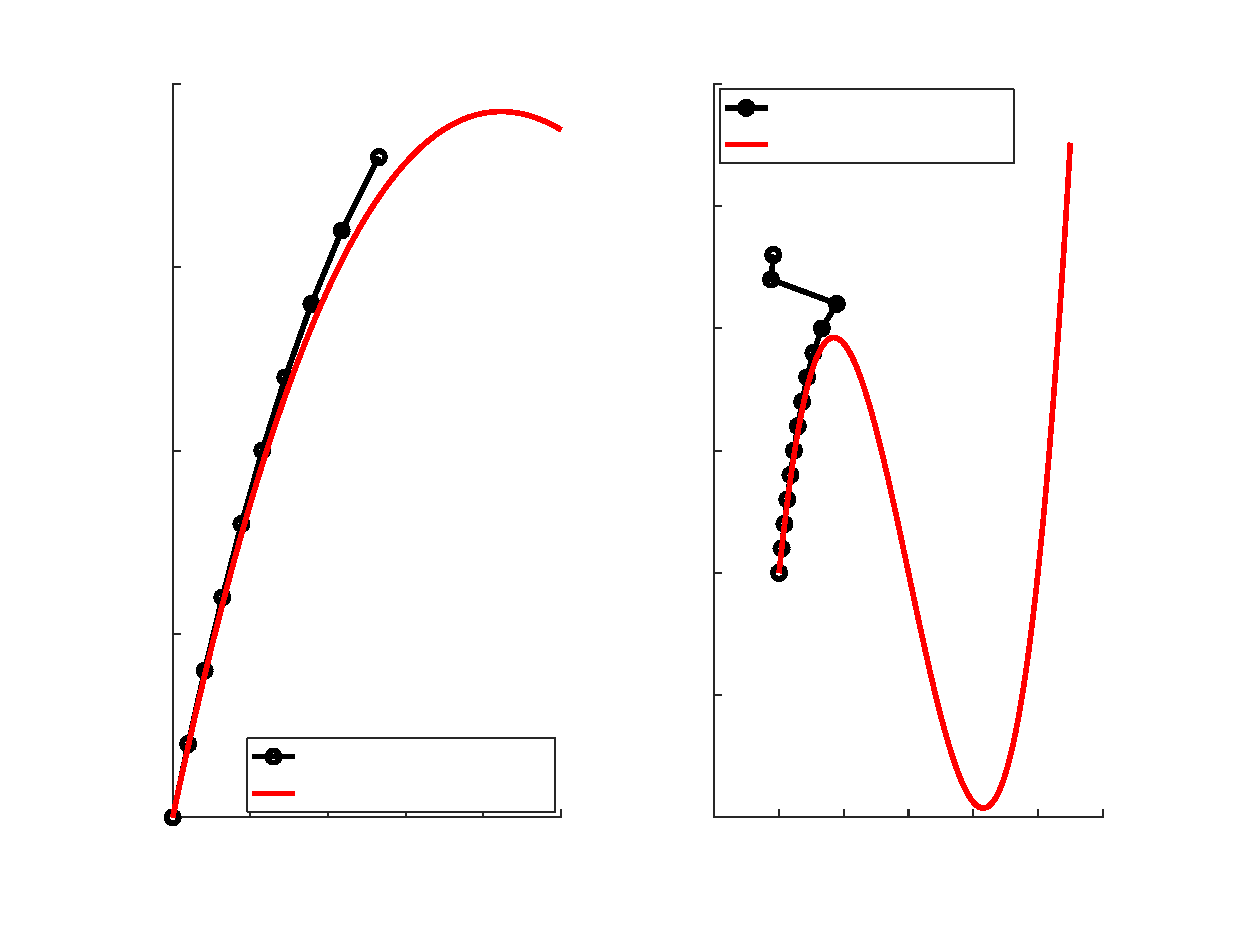
\includegraphics{Fig1Epscargabaja-inc}
\end{picture}%
\begin{picture}(576,432)(0,0)
\fontsize{15}{0}
\selectfont\put(74.88,42.5189){\makebox(0,0)[t]{\textcolor[rgb]{0.15,0.15,0.15}{{0}}}}
\fontsize{15}{0}
\selectfont\put(112.16,42.5189){\makebox(0,0)[t]{\textcolor[rgb]{0.15,0.15,0.15}{{0.1}}}}
\fontsize{15}{0}
\selectfont\put(149.44,42.5189){\makebox(0,0)[t]{\textcolor[rgb]{0.15,0.15,0.15}{{0.2}}}}
\fontsize{15}{0}
\selectfont\put(186.72,42.5189){\makebox(0,0)[t]{\textcolor[rgb]{0.15,0.15,0.15}{{0.3}}}}
\fontsize{15}{0}
\selectfont\put(224,42.5189){\makebox(0,0)[t]{\textcolor[rgb]{0.15,0.15,0.15}{{0.4}}}}
\fontsize{15}{0}
\selectfont\put(261.279,42.5189){\makebox(0,0)[t]{\textcolor[rgb]{0.15,0.15,0.15}{{0.5}}}}
\fontsize{15}{0}
\selectfont\put(69.8693,47.52){\makebox(0,0)[r]{\textcolor[rgb]{0.15,0.15,0.15}{{0}}}}
\fontsize{15}{0}
\selectfont\put(69.8693,135.54){\makebox(0,0)[r]{\textcolor[rgb]{0.15,0.15,0.15}{{0.05}}}}
\fontsize{15}{0}
\selectfont\put(69.8693,223.56){\makebox(0,0)[r]{\textcolor[rgb]{0.15,0.15,0.15}{{0.1}}}}
\fontsize{15}{0}
\selectfont\put(69.8693,311.58){\makebox(0,0)[r]{\textcolor[rgb]{0.15,0.15,0.15}{{0.15}}}}
\fontsize{15}{0}
\selectfont\put(69.8693,399.6){\makebox(0,0)[r]{\textcolor[rgb]{0.15,0.15,0.15}{{0.2}}}}
\fontsize{14}{0}
\selectfont\put(168.08,24.5188){\makebox(0,0)[t]{\textcolor[rgb]{0.15,0.15,0.15}{{$x$}}}}
\fontsize{14}{0}
\selectfont\put(30.8693,223.56){\rotatebox{90}{\makebox(0,0)[b]{\textcolor[rgb]{0.15,0.15,0.15}{{$\lambda$}}}}}
\fontsize{12}{0}
\selectfont\put(135.946,76.6871){\makebox(0,0)[l]{\textcolor[rgb]{0,0,0}{{Solución Num\'erica}}}}
\fontsize{12}{0}
\selectfont\put(135.946,59.0203){\makebox(0,0)[l]{\textcolor[rgb]{0,0,0}{{Solución Exacta}}}}
\fontsize{15}{0}
\selectfont\put(334.88,42.5189){\makebox(0,0)[t]{\textcolor[rgb]{0.15,0.15,0.15}{{-0.5}}}}
\fontsize{15}{0}
\selectfont\put(365.947,42.5189){\makebox(0,0)[t]{\textcolor[rgb]{0.15,0.15,0.15}{{0}}}}
\fontsize{15}{0}
\selectfont\put(397.014,42.5189){\makebox(0,0)[t]{\textcolor[rgb]{0.15,0.15,0.15}{{0.5}}}}
\fontsize{15}{0}
\selectfont\put(428.08,42.5189){\makebox(0,0)[t]{\textcolor[rgb]{0.15,0.15,0.15}{{1}}}}
\fontsize{15}{0}
\selectfont\put(459.147,42.5189){\makebox(0,0)[t]{\textcolor[rgb]{0.15,0.15,0.15}{{1.5}}}}
\fontsize{15}{0}
\selectfont\put(490.213,42.5189){\makebox(0,0)[t]{\textcolor[rgb]{0.15,0.15,0.15}{{2}}}}
\fontsize{15}{0}
\selectfont\put(521.28,42.5189){\makebox(0,0)[t]{\textcolor[rgb]{0.15,0.15,0.15}{{2.5}}}}
\fontsize{15}{0}
\selectfont\put(329.87,47.52){\makebox(0,0)[r]{\textcolor[rgb]{0.15,0.15,0.15}{{-0.2}}}}
\fontsize{15}{0}
\selectfont\put(329.87,106.2){\makebox(0,0)[r]{\textcolor[rgb]{0.15,0.15,0.15}{{-0.1}}}}
\fontsize{15}{0}
\selectfont\put(329.87,164.88){\makebox(0,0)[r]{\textcolor[rgb]{0.15,0.15,0.15}{{0}}}}
\fontsize{15}{0}
\selectfont\put(329.87,223.56){\makebox(0,0)[r]{\textcolor[rgb]{0.15,0.15,0.15}{{0.1}}}}
\fontsize{15}{0}
\selectfont\put(329.87,282.24){\makebox(0,0)[r]{\textcolor[rgb]{0.15,0.15,0.15}{{0.2}}}}
\fontsize{15}{0}
\selectfont\put(329.87,340.92){\makebox(0,0)[r]{\textcolor[rgb]{0.15,0.15,0.15}{{0.3}}}}
\fontsize{15}{0}
\selectfont\put(329.87,399.6){\makebox(0,0)[r]{\textcolor[rgb]{0.15,0.15,0.15}{{0.4}}}}
\fontsize{14}{0}
\selectfont\put(428.08,24.5189){\makebox(0,0)[t]{\textcolor[rgb]{0.15,0.15,0.15}{{$x$}}}}
\fontsize{14}{0}
\selectfont\put(295.87,223.56){\rotatebox{90}{\makebox(0,0)[b]{\textcolor[rgb]{0.15,0.15,0.15}{{$\lambda$}}}}}
\fontsize{12}{0}
\selectfont\put(362.882,388.1){\makebox(0,0)[l]{\textcolor[rgb]{0,0,0}{{Solución Numérica}}}}
\fontsize{12}{0}
\selectfont\put(362.882,370.433){\makebox(0,0)[l]{\textcolor[rgb]{0,0,0}{{Solución Exacta}}}}
\end{picture}
}
	%	\includegraphics[width=1\linewidth]{sourcesJBBG/Fig1}
	\caption{Soluciones obtenidas usando Euler Hacia Adelante. Izquierda: solución para $\lambda^*=0.18$. Derecha: solución para $\lambda^*=0.26$.}
	\label{fig:fig1}
\end{figure}

Los resultados obtenidos permiten establecer que el método incremental descrito tiene dificultades para resolver el sistema más allá de puntos en los cuales se cumple que: $\det(\bfF_x)=0$ ($f'=0$ en este caso). %
%
Por otra parte el efecto de \textit{drift} puede provocar que las soluciones tengan errores considerables si el incremento no es cuidadosamente seleccionado. %
%
Estas desventajas del método motivan a introducir los métodos iterativos en la siguiente sección.



\lstinputlisting[caption = {Implementación del Método de Euler para Ejemplo Numérico 1.}\label{cod:ejnonlin}]{../src/Incremental1dof.m}
%
%
\subsection{Métodos Iterativos}\label{Iter}

Luego de haber presentado los métodos incrementales y observar desventajas como el fenómeno de \textit{drift}, se plantea en esta sección la resolución del problema en cuestión por medio de métodos iterativos. %

La idea fundamental de los métodos iterativos es fijar el valor del parámetro $\lambda=\lambda_k$ y hallar el vector $\bfx_k$ que verifica la ecuación no lineal: $\bff(\bfx_k)-\lambda_k \bfv=0$. De esta manera las incógnitas del sistema no lineal son solamente las entradas del vector $\bfx_k$.

El procedimiento consiste en, dado un vector inicial $\bfx_k^{(0)}$, iterar mediante alguna regla de manera de asegurar que el vector obtenido ($\bfx_k^{(N)}$) satisface la ecuación no lineal con una tolerancia definida a priori, siendo $N$ el número de iteraciones requeridas. %
%
La expresión matemática asociada a satisfacer la ecuación no lineal es:
%
\begin{equation}\label{ec9}
	\| \bff(\bfx_k^{(N)}) - \lambda_k \bfv \| < \epsilon_{tol}.
\end{equation}

Este procedimiento iterativo suele llamarse ``iterar hasta obtener convergencia''. %
%
Iterar hasta satisfacer la condición dada por la Ecuación~\eqref{ec9} garantiza que se habrá obtenido un punto $(\lambda_k,\bfx_k^{(N)})$ para el cual se tiene un error controlado respecto de la solución exacta. Es por esto que los métodos iterativos eliminan el problema de \textit{drift}.



A continuación se presenta una de las reglas iterativas más populares para resolver sistemas de ecuaciones no lineales, el llamado Método de Newton-Raphson.

\subsubsection{Método de Newton-Raphson} \label{sec:NRcap1}

En el Método de Newton-Raphson (NR) se asume que se cuenta con un vector $\bfx_k^{(0)}$ próximo a la solución buscada $\bfx_k$ de la Ecuación~\eqref{ec2}. Para una ecuación no lineal con una sola incógnita, el método se puede deducir mediante un argumento geométrico, mientras que para un sistema de ecuaciones no lineales, la deducción requiere del concepto de linealización de funciones vectoriales.

A modo de referencia, el software SAP 2000\textsuperscript{\textregistered} \footnote{desarrollado por \textit{Computers and Structures Inc.}}, utiliza iteraciones de N-R para resolver problemas con no linealidad geométrica, permitiendo al usuario definir parámetros básicos del método.


\paragraph{Una Ecuación y Una Variable:} %
%
Se describe a continuación la deducción geométrica para el caso de una sola incógnita. De acuerdo a lo que se muestra en la Figura~\ref{fig:fig2}, la idea del método es trazar la tangente a la curva $(x,f(x))$ en el punto conocido $x_k^{(0)}$ y hallar la intersección de esta recta tangente con la recta horizontal dada por el nivel de carga definido: $\lambda_k \bfv$. %
%
El valor de $x$ en esta intersección será la nueva aproximación de la solución de la ecuación no lineal $x_k^{(1)}$.

\begin{figure}[htb]
	\centering
   \def\svgwidth{0.7\textwidth}
\input{../fig/esquemaIterNR.pdf_tex}
	\caption{Representación geométrica de iteración de Newton-Raphson.}
	\label{fig:fig2}
\end{figure}

La ecuación de recta de la tangente en el punto $x_k^{(0)}$ está dada por:
%
\begin{equation}
	\lambda v = f(x_k^{(0)})+f'(x_k^{(0)})(x-x_k^{(0)}),
\end{equation}
%
mientras que la ecuación de la recta horizontal correspondiente al nivel de carga especificado es:
%
\begin{equation}
	\lambda v = \lambda_k v.
\end{equation}

La intersección de ambas rectas provee la siguiente ecuación lineal en $x$:
%
\begin{equation}
\lambda_k v = f(x_k^{(0)})+f'(x_k^{(0)})(x-x_k^{(0)}).
\end{equation}

Resolviendo $x$ en la ecuación anterior y definiendo ese valor como la nueva aproximación de la solución: $x_k^{(1)}$,
se llega a:
%
\begin{equation}
x_k^{(1)}=x_k^{(0)}-\frac{f(x_k^{(0)})-\lambda_k v}{f'(x_k^{(0)})}.
\end{equation}

El procedimiento anterior permite definir el método iterativo de Newton-Raphson:
%
\begin{equation}\label{NR1}
\text{N-R}
	\begin{cases} 
	\displaystyle
		x_k^{(i+1)}=x_k^{(i)}-\frac{f(x_k^{(i)})-\lambda_k v}{f'(x_k^{(i)})} \\
		x_k^{(0)}
	\end{cases}
\end{equation}

Es claro a partir de la Ecuación~\eqref{NR1} que este método no puede iterar si la derivada primera de $f(x)$ es igual a cero en el punto donde se traza la tangente. Esta limitación también estará presente en el caso de Newton-Raphson para varias variables.


\paragraph{Sistema de $n$ Ecuaciones y $n$ Variables:} %
%
A continuación se presenta la deducción del método de Newton-Raphson para un sistema de $n$ ecuaciones no lineales con $n$ incógnitas. Se trabajará con el sistema de ecuaciones no lineales dado en la Ecuación~\eqref{ec3}. %
%
Para deducir el método, se linealiza el sistema de ecuaciones no lineales en el punto actual de la iteración $\bfx_k^{(i)}$. Esto se efectúa mediante un desarrollo de Taylor de $\bff$ respecto de la variable $\bfx$ en un entorno de $\bfx_{k}^{(i)}$:
%
\begin{equation}
	\lambda \bfv = \bff(\bfx_k^{(i)})+\bfF_x(\bfx_k^{(i)})(\bfx-\bfx_k^{(i)})+O(\|\bfx-\bfx_k^{(i)}\|^2)
\end{equation}

Imponiendo que $\lambda \bfv=\lambda_k \bfv$ y truncando el término de mayor orden se obtiene un sistema de ecuaciones  lineales en la variable $\bfx$:
%
\begin{equation}\label{ec10}
\lambda_k \bfv = \bff(\bfx_k^{(i)})+\bfF_x(\bfx_k^{(i)})(\bfx-\bfx_k^{(i)})
\end{equation}

Se define el paso del método de Newton-Raphson como $\Delta \bfx_k^{(i)}=\bfx_k^{(i+1)}-\bfx_k^{(i)}$ y a partir de la Ecuación~\eqref{ec10} se obtiene:
%
\begin{equation}\label{NR2}
\text{N-R}
\begin{cases} 
	\bfF_x(\bfx_k^{(i)})\Delta \bfx_k^{(i)} =-\left((\bff(\bfx_k^{(i)})-\lambda_k \bfv\right)\\
	\bfx_k^{(i+1)}=\bfx_k^{(i)}+\Delta \bfx_k^{(i)} \\
	\bfx_k^{(0)}
\end{cases}
\end{equation}

\cajaactividad{
Verificar que si $x\in\mathbb{R}$ el método dado por la Ecuación~\eqref{NR2} se reduce al presentado en la Ecuación~\eqref{NR1}.}

Asumiendo que el punto de arranque ($\bfx_k^{(0)}$) está suficientemente cerca de la solución buscada, la sucesión de iterados que genera N-R converge con orden 2. Esto significa que las distancias entre cada iterado y la solución exacta ($\bfx_k$) verifican $\|\bfx_k^{(i+1)}-\bfx_k\| \approx \beta \|\bfx_k^{(i)}-\bfx_k\|^2$, siendo $\beta>0$ la velocidad de convergencia. %
%
En este documento no se presentarán formalmente los conceptos de orden y velocidad de convergencia, ver \citep{quarteroni2007numeric} por dichas definiciones.

El método de N-R presentado en (\ref{NR2}) requiere que $\bfF_x(\bfx_k^{(i)})$ sea invertible para poder calcular el paso iterativo. Más en general, para poder tener pasos iterativos con precisión confiable se deberá cumplir que el número de condición de la matriz $\bfF_x(\bfx_k^{(i)})$ sea pequeño. Ver la Sección 7.6 del libro \citep{dahquist2008numeric} por más detalles sobre estimación de número de condición, perturbaciones y errores en sistemas lineales.

En la introducción a los métodos iterativos, en la Sección \ref{Iter}, se introdujo un criterio de parada general, el cual es válido evidentemente para la iteración de N-R. Existen otros posibles criterios de parada, como por ejemplo fijar un límite máximo para el número de iteraciones: $i\leq \text{MAXITER}$. Otro criterio puede ser iterar hasta que la diferencia relativa entre dos iterados sea menor que una tolerancia $\epsilon_{rel}$:
%
\begin{equation}
	\frac{\|\Delta \bfx_k^{(i)}\|}{\|\bfx_k^{(i+1)}\|} < \epsilon_{rel}
\end{equation}

En cada iteración de N-R se debe resolver un sistema de tamaño $(n \times n)$. Dependiendo de la estructura de la matriz $\bfF_x(x_k^{(i)})$ esta solución puede llevarse a cabo de maneras más eficientes que una escalerización de Gauss genérica. En el capítulo 8 de \citep{Bathe2014} se pueden ver en detalle métodos numéricos eficientes usados para la solución de dichos sistemas lineales.

La evaluación de la matriz $\bfF_x$ y su factorización (solución del sistema lineal) en cada paso de N-R tiene un costo elevado. Existen otros métodos numéricos iterativos que evitan evaluar $\bfF_x$ en cada iteración, o que utilizan una definición distinta para $\bfF_x$ de manera de obtener solución con menor costo computacional en cada iteración.

\subsubsection{Método de Newton-Raphson Modificado}

El método de N-R modificado presenta una alternativa para no tener que evaluar y factorizar la matriz $\bfF_x$ en cada iteración. Precisamente esto es lo que define al método en cuestión, el mismo deja fija la matriz $\bfF_x(\bfx_k^{(0)})$ a lo largo de las iteraciones.

Algunas herramientas computacionales, como por ejemplo el software SAP 2000\textsuperscript{\textregistered}, resuelven problemas con no linealidad geométrica realizando un cierto número de iteraciones de NR modificado para luego pasar a realizar iteraciones Newton-Raphson si no se alcanza convergencia.

La iteración de Newton-Raphson modificado puede ser escrita como:
%
\begin{equation}\label{NRM}
\text{N-R Modif.}
\begin{cases} 
\bfF_x(\bfx_k^{(0)})\Delta \bfx_k^{(i)} =-\left((\bff(\bfx_k^{(i)})-\lambda_k \bfv\right)\\
\bfx_k^{(i+1)}=\bfx_k^{(i)}+\Delta \bfx_k^{(i)} \\
\bfx_k^{(0)}
\end{cases}
\end{equation}

Esto permite factorizar la matriz $\bfF_x(\bfx_k^{(0)})$ al comienzo de las iteraciones y almacenar dichos factores. Luego, en cada paso iterativo se deberá resolver una sustitución hacia adelante y una sustitución hacia atrás para hallar $\Delta \bfx_k^{(i)}$. El costo computacional de dichas sustituciones es un orden de magnitud menor (en $n$) que el de la factorización de la matriz $\bfF_x(\bfx_k^{(0)})$.

Como contrapartida al costo computacional reducido de N-R Modificado, se destaca que el orden de convergencia del método es 1. Esto implica que las distancias entre cada iterado y la solución exacta ($\bfx_k$) verifican $\|\bfx_k^{(i+1)}-\bfx_k\| \approx \beta \|\bfx_k^{(i)}-\bfx_k\|$, con $\beta \in (0,1)$.

\subsubsection{Métodos Cuasi-Newton}

La familia de métodos cuasi-Newton comprende a aquellos en los cuales se cambia la matriz $\bfF_x$ del método de Newton-Raphson (matriz tangente) por una matriz más económica de evaluar y factorizar (matriz secante).

En el caso de una sola ecuación y una sola incógnita, el Método de la Secante corresponde a un método cuasi-Newton. %
%
En éste método, en lugar de trazar la tangente por el punto actual ($x_k^{(i)}$), se traza la secante por el punto actual y el anterior como se muestra en la Figura \ref{fig:fig3}.
%
\begin{figure}[htb]
	\centering
   \def\svgwidth{0.7\textwidth}
\input{../fig/esquemaIterQN.pdf_tex}
	\caption{Esquema Geométrico del Método de la Secante}
	\label{fig:fig3}
\end{figure}

Es claro que se deben especificar dos puntos de arranque para poder comenzar a iterar con el Método de la Secante.

\cajaactividad{
Verificar que la expresión de la iteración del Método de la secante está dada por:
%
\begin{equation}
	x_k^{(i+1)}=x_k^{(i)} -\frac{x_k^{(i)}-x_k^{(i-1)}}{f(x_k^{(i)})-f(x_k^{(i-1)})}\left(f(x_k^{(i)})-\lambda_k \bfv \right)
\end{equation}
}

El Método de la Secante tiene orden de convergencia super-lineal ($\text{Orden}=\frac{1+\sqrt{5}}{2}$), lo cual lo posiciona como más lento que N-R pero más rápido que N-R Modificado.

La generalización del Método de la Secante a sistemas de ecuaciones no lineales corresponde al Método de Broyden. %
%
En ese método, en lugar de la matriz tangente $\bfF_x$ utilizada en N-R, se utiliza una matriz secante que verifica una relación en los incrementos de $\bff(\bfx)$ y $\bfx$ de la forma: $\Delta \bff_k = \bfB_k \Delta \bfx_k$. La condición de matriz secante no es suficiente para definir la completamente y es ahí donde surgen distintas variantes. %
%
En la Sección 7.1.4 de \citep{quarteroni2007numeric} se presenta una definición más detallada del método. %

Otro método cuasi-Newton que deriva de la condición secante mencionada anteriormente es el Método BFGS, cuya formulación puede encontrarse en la Sección 8.4.2 de \citep{Bathe2014}.

El motivo por el cual estos métodos son atractivos es que en ellos las inversas de las matrices secantes se actualizan de forma computacionalmente económica a partir de las anteriores. Se obtiene, por lo tanto, un compromiso entre velocidad y economía computacional.

\subsubsection{Ejemplo Numérico 2: Soluciones Iterativas}

Se resuelve nuevamente la ecuación no lineal vista en el ejemplo dado en la Sección~\ref{ej1}, dada por la expresión:
%
\begin{equation}
x-\frac{3}{2}x^2+\frac{1}{2}x^3-\lambda=0
\end{equation}

En este caso se fija el nivel de carga $\lambda_k=0.19$ y se comienza la iteración desde $x_k^{(0)}=0$. %
%
La expresión del Método de Newton-Raphson para la ecuación no lineal a resolver está dada por:
%
\begin{equation}
x_k^{(i+1)}=x_k^{(i)}-\frac{x_k^{(i)}-\frac{3}{2}{x_k^{(i)}}^2+\frac{1}{2}{x_k^{(i)}}^3-0.19 }{1-3x_k^{(i)}+\frac{3}{2}{x_k^{(i)}}^2},
\end{equation}
%
mientras que la iteración del Método de Newton-Raphson Modificado está dada por:
%
\begin{equation}
x_k^{(i+1)}=x_k^{(i)}-\frac{x_k^{(i)}-\frac{3}{2}{x_k^{(i)}}^2+\frac{1}{2}{x_k^{(i)}}^3-0.19 }{1}.
\end{equation}

La implementación de ambos métodos se presenta al final de esta sección, en el Código \ref{cod:EjNum2}. %
%
En la Figura~\ref{fig:fig4} se muestran resultados obtenidos al aplicar los métodos a la resolución del ejemplo considerando $\epsilon_{tol}=10^{-8}$. %
%

\begin{figure}[htb]
	\centering
	\resizebox{\textwidth}{!}{% Title: gl2ps_renderer figure
% Creator: GL2PS 1.4.0, (C) 1999-2017 C. Geuzaine
% For: Octave
% CreationDate: Fri Dec 29 11:28:09 2017
\setlength{\unitlength}{1pt}
\begin{picture}(0,0)
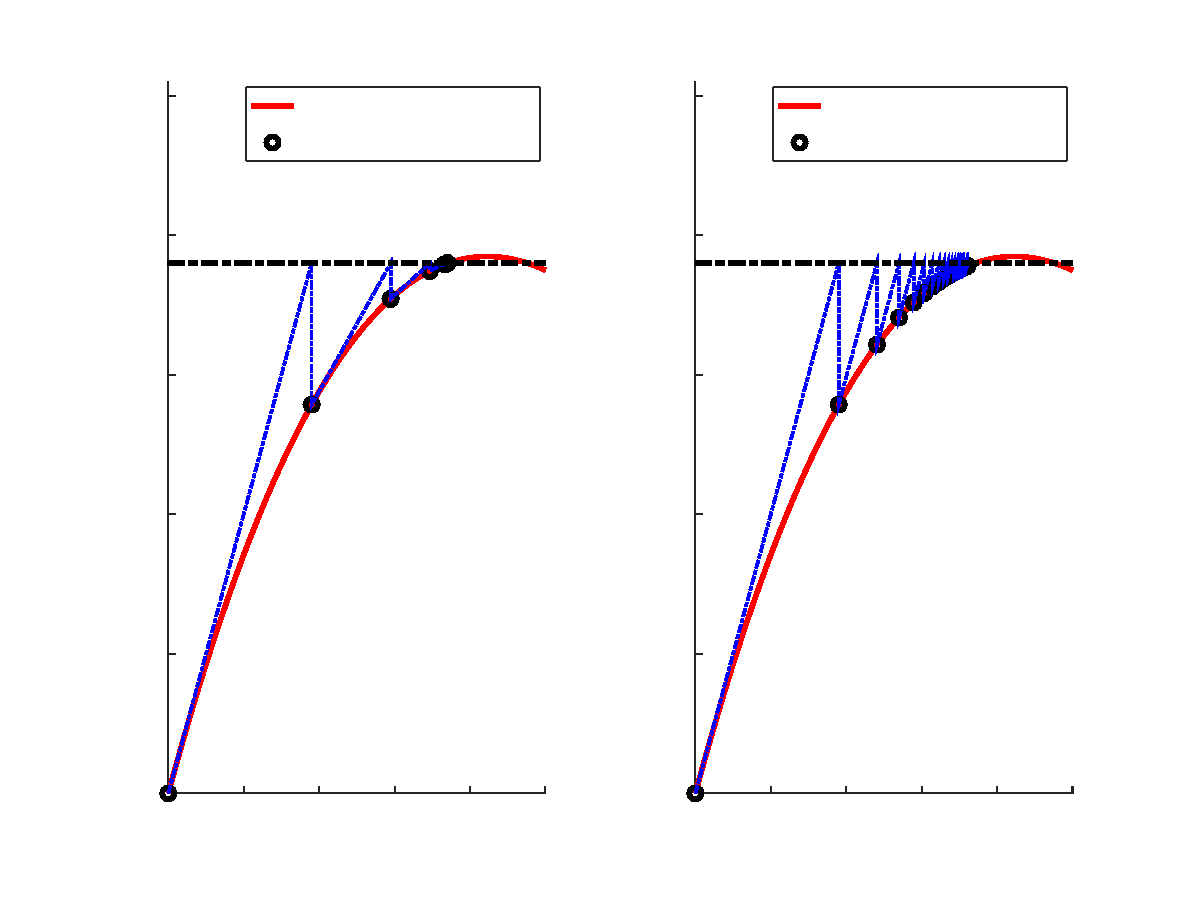
\includegraphics{Fig4Epscargabaja-inc}
\end{picture}%
\begin{picture}(560,419)(0,0)
\fontsize{15}{0}
\selectfont\put(72.8,41.0829){\makebox(0,0)[t]{\textcolor[rgb]{0.15,0.15,0.15}{{0}}}}
\fontsize{15}{0}
\selectfont\put(109,41.0829){\makebox(0,0)[t]{\textcolor[rgb]{0.15,0.15,0.15}{{0.1}}}}
\fontsize{15}{0}
\selectfont\put(145.2,41.0829){\makebox(0,0)[t]{\textcolor[rgb]{0.15,0.15,0.15}{{0.2}}}}
\fontsize{15}{0}
\selectfont\put(181.4,41.0829){\makebox(0,0)[t]{\textcolor[rgb]{0.15,0.15,0.15}{{0.3}}}}
\fontsize{15}{0}
\selectfont\put(217.6,41.0829){\makebox(0,0)[t]{\textcolor[rgb]{0.15,0.15,0.15}{{0.4}}}}
\fontsize{15}{0}
\selectfont\put(253.799,41.0829){\makebox(0,0)[t]{\textcolor[rgb]{0.15,0.15,0.15}{{0.5}}}}
\fontsize{15}{0}
\selectfont\put(67.8,46.09){\makebox(0,0)[r]{\textcolor[rgb]{0.15,0.15,0.15}{{0}}}}
\fontsize{15}{0}
\selectfont\put(67.8,113.048){\makebox(0,0)[r]{\textcolor[rgb]{0.15,0.15,0.15}{{0.05}}}}
\fontsize{15}{0}
\selectfont\put(67.8,180.006){\makebox(0,0)[r]{\textcolor[rgb]{0.15,0.15,0.15}{{0.1}}}}
\fontsize{15}{0}
\selectfont\put(67.8,246.964){\makebox(0,0)[r]{\textcolor[rgb]{0.15,0.15,0.15}{{0.15}}}}
\fontsize{15}{0}
\selectfont\put(67.8,313.921){\makebox(0,0)[r]{\textcolor[rgb]{0.15,0.15,0.15}{{0.2}}}}
\fontsize{15}{0}
\selectfont\put(67.8,380.879){\makebox(0,0)[r]{\textcolor[rgb]{0.15,0.15,0.15}{{0.25}}}}
\fontsize{14}{0}
\selectfont\put(163.3,23.0829){\makebox(0,0)[t]{\textcolor[rgb]{0.15,0.15,0.15}{{$x$}}}}
\fontsize{14}{0}
\selectfont\put(28.8,216.832){\rotatebox{90}{\makebox(0,0)[b]{\textcolor[rgb]{0.15,0.15,0.15}{{$\lambda$}}}}}
\fontsize{12}{0}
\selectfont\put(135.466,376.102){\makebox(0,0)[l]{\textcolor[rgb]{0,0,0}{{Solución Exacta}}}}
\fontsize{12}{0}
\selectfont\put(135.466,358.477){\makebox(0,0)[l]{\textcolor[rgb]{0,0,0}{{Solución Numérica}}}}
\fontsize{15}{0}
\selectfont\put(325.801,41.0829){\makebox(0,0)[t]{\textcolor[rgb]{0.15,0.15,0.15}{{0}}}}
\fontsize{15}{0}
\selectfont\put(362,41.0829){\makebox(0,0)[t]{\textcolor[rgb]{0.15,0.15,0.15}{{0.1}}}}
\fontsize{15}{0}
\selectfont\put(398.2,41.0829){\makebox(0,0)[t]{\textcolor[rgb]{0.15,0.15,0.15}{{0.2}}}}
\fontsize{15}{0}
\selectfont\put(434.4,41.0829){\makebox(0,0)[t]{\textcolor[rgb]{0.15,0.15,0.15}{{0.3}}}}
\fontsize{15}{0}
\selectfont\put(470.6,41.0829){\makebox(0,0)[t]{\textcolor[rgb]{0.15,0.15,0.15}{{0.4}}}}
\fontsize{15}{0}
\selectfont\put(506.8,41.0829){\makebox(0,0)[t]{\textcolor[rgb]{0.15,0.15,0.15}{{0.5}}}}
\fontsize{15}{0}
\selectfont\put(320.801,46.09){\makebox(0,0)[r]{\textcolor[rgb]{0.15,0.15,0.15}{{0}}}}
\fontsize{15}{0}
\selectfont\put(320.801,113.048){\makebox(0,0)[r]{\textcolor[rgb]{0.15,0.15,0.15}{{0.05}}}}
\fontsize{15}{0}
\selectfont\put(320.801,180.006){\makebox(0,0)[r]{\textcolor[rgb]{0.15,0.15,0.15}{{0.1}}}}
\fontsize{15}{0}
\selectfont\put(320.801,246.964){\makebox(0,0)[r]{\textcolor[rgb]{0.15,0.15,0.15}{{0.15}}}}
\fontsize{15}{0}
\selectfont\put(320.801,313.921){\makebox(0,0)[r]{\textcolor[rgb]{0.15,0.15,0.15}{{0.2}}}}
\fontsize{15}{0}
\selectfont\put(320.801,380.879){\makebox(0,0)[r]{\textcolor[rgb]{0.15,0.15,0.15}{{0.25}}}}
\fontsize{14}{0}
\selectfont\put(416.3,23.0829){\makebox(0,0)[t]{\textcolor[rgb]{0.15,0.15,0.15}{{$x$}}}}
\fontsize{14}{0}
\selectfont\put(281.801,216.832){\rotatebox{90}{\makebox(0,0)[b]{\textcolor[rgb]{0.15,0.15,0.15}{{$\lambda$}}}}}
\fontsize{12}{0}
\selectfont\put(388.466,376.102){\makebox(0,0)[l]{\textcolor[rgb]{0,0,0}{{Solución Exacta}}}}
\fontsize{12}{0}
\selectfont\put(388.466,358.477){\makebox(0,0)[l]{\textcolor[rgb]{0,0,0}{{Solución Numérica}}}}
\end{picture}
}
%	\includegraphics[width=.9\linewidth]{sourcesJBBG/Fig4}
	\caption{Resultados obtenidos por métodos iterativos. Izquierda: método de Newton-Raphson. Derecha: método de Newton-Raphson Modificado.}
	\label{fig:fig4}
\end{figure}

El método Newton-Raphson Modificado requiere 20 iteraciones mientras que el método Newton-Raphson requiere 7. %
%
Vale la pena remarcar que, dado que $f'(x)$ en la solución tiene un valor cercano a cero, el método requiere un número de iteraciones considerablemente elevado para converger. %
%
Esto se puede comprender mejor si se tiene en cuenta el siguiente resultado teórico: el método de N-R tiene orden de convergencia igual a 1 cuando $f'(x)$ en la raíz es igual a 0.

\cajaactividad{Modificar los parámetros de la implementación presentada y resolver el ejemplo para $\lambda_{k}=0.26$ y otros dos valores superiores a $0.2$. %
%
Analizar los resultados y comparar con los obtenidos por el método incremental.}

\lstinputlisting[caption = {Implementación de métodos iterativos para ejemplo numérico 2.}\label{cod:EjNum2}]{../src/Iterative1dof.m}


\subsection{Métodos de Longitud de Arco (Arc-Length)}\label{ArcLength}

En esta sección se presenta una variante de Método de Longitud de Arco para la resolución de sistemas de ecuaciones no lineales parametrizados del tipo dado en la Ecuación~\eqref{ec3}. %
%
Estos métodos son estudiados en matemática aplicada en el área de continuación numérica (ver notas del curso de \textit{Análisis numérico de ecuaciones no-lineales} \citep{Doedl2014Slides} y el software AUTO-07p \citep{AUTO-07p}). %
%
Por otra parte, se destaca que estos métodos fueron inicialmente desarrollados en el área de análisis estructural. %
%
Una breve reseña histórica puede encontrarse en la Sección 9.3 de \citep{crisfield1996non}. 

La ventaja fundamental de estos métodos sobre los expuestos en las secciones anteriores es que los Métodos de Longitud de Arco permiten resolver las ecuaciones no lineales en situaciones en las cuales los métodos anteriores fallan o encuentran problemas de convergencia.

Del punto de vista estructural, el interés en poder resolver el equilibrio de estructuras más allá de puntos críticos o puntos de soluciones con matriz tangente singular (más detalles en Capítulo~\ref{cap2GNA}) se justifica en que:
%
\begin{itemize}
	\item Puede ocurrir que un punto crítico solamente sea un máximo local de la curva de carga-desplazamiento.
	\item Puede ocurrir que se desee analizar un componente asilado de una estructura, para luego incorporar ese componente a una estructura completa.
	\item En general es importante saber cual es la carga de colapso de una estructura, pero además es importante saber como es su comportamiento post-colapso, si es dúctil o frágil por ejemplo.
	\item Para saber que efectivamente se alcanzó la capacidad de carga máxima de la estructura, se debe ser capaz de resolver el equilibrio más allá de dicho punto para poder verificar que en efecto es un máximo.
	\item Para poder estudiar el estado de tensiones que la estructura tiene en su carga de colapso, se debe ser capaz de converger la solución en dicho punto de carga máxima. Esto es difícil con los métodos presentados anteriormente.
	\item En la solución de problemas elásticos-perfectamente plásticos, la carga máxima de la estructura (capacidad plástica) es difícil de obtener mediante los métodos anteriores dado que la curva de carga-desplazamiento alcanza una meseta plástica en dicha carga.
\end{itemize}

Es claro a partir de lo anterior que estos métodos son esenciales para el análisis computacional del colapso de estructuras. Algunas herramientas computacionales como: ABAQUS\textsuperscript{\textregistered}, LUSAS\textsuperscript{\textregistered}, ANSYS\textsuperscript{\textregistered} o ADINA\textsuperscript{\textregistered} tienen la capacidad de llevar a cabo análisis estáticos mediante este tipo de procedimientos.

En lo que sigue se presenta una versión básica del método de Longitud de Arco, la cual no es una implementación eficiente pero tiene como ventaja la claridad en su formulación. En la Sección 9.3 de \citep{crisfield1996non} se presenta una exposición completa de estos métodos y su historia.

La idea básica de estos métodos es considerar a $\bfx\in\mathbb{R}^n$ y $\lambda\in\mathbb{R}^+$ como incógnitas. Se requiere, naturalmente, que esas incógnitas satisfagan la Ecuación~\eqref{ec3}. %
%
Sin embargo, ésta condición por sí sola no es suficiente para tener un problema determinado, ya que se puede comprobar que en ese caso se tienen $n+1$ incógnitas y $n$ ecuaciones. Por lo tanto, los métodos de Longitud de Arco imponen una restricción adicional de manera de obtener un problema determinado.

Dependiendo de cuál sea dicha restricción adicional y la implementación elegida, se obtienen los distintos métodos que forman parte de la familia de Métodos de longitud de arco. Ver en \citep{crisfield1996non} Métodos de Longitud de Arco Linealizado, Cilíndrico y Esférico. %
%
La restricción adicional está, tal como lo indica el nombre de cada método, directamente relacionada al concepto de longitud del arco de la curva carga-desplazamiento. %
%
En la Figura~\ref{fig:fig5} se presenta un esquema geométrico de la restricción de longitud de arco. %


\begin{figure}[htb]
	\centering
   \def\svgwidth{0.65\textwidth}
\input{../fig/esquemaIterAL.pdf_tex}
	\caption{Esquema geométrico del Método de Longitud de Arco.}
	\label{fig:fig5}
\end{figure}

El incremento diferencial de la coordenada de longitud de arco $s$ puede escribirse en función de los incrementos de carga y desplazamiento como:
%
\begin{equation}
	ds^2 = \dif\bfx^T\dif\bfx+\dif\lambda^2 \psi^2 \bfv^T\bfv,
\end{equation}
%
donde $\psi$ es un factor de escala de la carga con respecto a los desplazamientos. %
%
Esta relación diferencial para la longitud de arco se puede traducir a una relación en los incrementos $\Delta \bfx$ y $\Delta \lambda$:
%
\begin{equation}\label{ec11}
\Delta l^2 = \Delta \bfx^T \Delta \bfx+\Delta \lambda^2 \psi^2 \bfv^T\bfv.
\end{equation}

Observar que el parámetro $\Delta l^2$ controla la distancia a la cual el método de Longitud de Arco busca el nuevo punto solución de la ecuación no lineal.

En lo que sigue, se asume que se tiene una solución de la ecuación $\left(\bfx_{k-1},\lambda_{k-1}\right)$ y que el arco de radio $\Delta l$ está centrado en ese punto. Con lo cual: $\Delta \bfx_k = \bfx_k - \bfx_{k-1} $ y $\Delta \lambda_k = \lambda_k - \lambda_{k-1}$.

De esta manera el sistema de ecuaciones no lineales que se deberán satisfacer en el método de Longitud de Arco propuesto son:
%
\begin{equation}\label{ec12}
\begin{cases} 
\bff(\bfx_k) - \lambda_k \bfv = 0\\
\Delta \bfx_k^T \Delta \bfx_k+\Delta \lambda_k^2 \psi^2 \bfv^T\bfv - \Delta l^2 = 0 \\
\end{cases}
\end{equation}

Para obtener la expresión de la iteración del método de Longitud de Arco se debe linealizar las ecuaciones no lineales dadas en la Ecuación~\eqref{ec12} en torno al último punto iterado: 
$$\left(\bfx_{k-1}+\Delta \bfx_k^{(i)}, \lambda_{k-1}+\Delta \lambda_k^{(i)}\right)$$  respecto de las incógnitas $\Delta \bfx_k$ y $\Delta \lambda_k$.

Luego, se resuelve el sistema lineal resultante definiendo el paso iterativo del método. %
%
Notar que se expresa la linealización e iteraciones respecto de los incrementos de las variables $\bfx$ y $\lambda$.

Las ecuaciones linealizadas resultantes son:
%
%\begin{equation}\label{ec12b}
%\begin{cases} \begin{split}
%	\bff\left(\bfx_{k-1}+\Delta \bfx_k^{(i)}\right)- \left(\lambda_{k-1}+\Delta \lambda_k^{(i)}\right) \bfv +&\\
%	\bfF_x\left(\bfx_{k-1} +\Delta \bfx_k^{(i)}\right)&\delta \bfx_k^{(i)} - \delta \lambda_k^{(i)} \bfv=0
%\end{split}\\ \\
%\begin{split}
%	{\Delta \bfx_k^{(i)}}^T \Delta \bfx_k^{(i)} + {\Delta \lambda_k^{(i)}}^2 \psi^2 \bfv^T\bfv - \Delta l^2  + &\\
%	2{\Delta \bfx_k^{(i)}}^T\delta \bfx_k^{(i)} + &2\psi^2\bfv^T\bfv\Delta \lambda_k^{(i)}\delta \lambda_k^{(i)}= 0
%\end{split} \\
%\end{cases}
%\end{equation}
%
\begin{small}
\begin{eqnarray}\label{ec12b}
\bff\!\left(\bfx_{k-1}+\Delta \bfx_k^{(i)}\right)\!-\!\left(\lambda_{k-1}+\Delta \lambda_k^{(i)}\right)\!\bfv\!+\!\bfF_x\!\left(\bfx_{k-1} +\Delta \bfx_k^{(i)}\right) \delta \bfx_k^{(i)} - \delta \lambda_k^{(i)} \bfv =\!0\\
{\Delta \bfx_k^{(i)}}^T \Delta \bfx_k^{(i)} + {\Delta \lambda_k^{(i)}}^2 \psi^2 \bfv^T\bfv - \Delta l^2 +
2{\Delta \bfx_k^{(i)}}^T\delta \bfx_k^{(i)} + 2\psi^2\bfv^T\bfv\Delta \lambda_k^{(i)}\delta \lambda_k^{(i)} = 0
\end{eqnarray}
%
\end{small}
con los incrementos iterativos definidos como
\begin{equation}\label{ec13}
		\delta \bfx_k^{(i)}=\Delta \bfx_k^{(i+1)}-\Delta \bfx_k^{(i)} \qquad \text{y} \qquad
		\delta \lambda_k^{(i)}=\Delta \lambda_k^{(i+1)}-\Delta \lambda_k^{(i)}		.
\end{equation}

La versión linealizada de la Ecuación~\eqref{ec12} se traduce en el siguiente sistema lineal a ser resuelto en cada iteración del método:
%
\begin{eqnarray}\label{ec14}
\left[\begin{array}{cc}
\bfF_x\left(\bfx_{k-1} +\Delta \bfx_k^{(i)}\right) & -\bfv\\ 
2 \left(\Delta \bfx_k^{(i)}\right)^{\text{T}} &  2\psi^2\bfv^{\text{T}}\bfv\Delta \lambda_k^{(i)} 
\end{array}\right] \cdot 
\left[\begin{array}{c} 
\delta \bfx_k^{(i)} \\
\delta \lambda_k^{(i)} 
\end{array}
\right] = \\ 
\dots 
\left[\begin{array}{c}
-\left( \bff\left(\bfx_{k-1}+\Delta \bfx_k^{(i)}\right)- \left(\lambda_{k-1}+\Delta \lambda_k^{(i)}\right) \bfv \right)\\
-\left(
    {\Delta \bfx_k^{(i)}}^{\text{T}}   \Delta \bfx_k^{(i)} 
  + {\Delta \lambda_k^{(i)}}^2 \psi^2 \bfv^{\text{T}}\bfv - \Delta l^2
\right)
\end{array}\right].
\end{eqnarray}

La regla para actualizar la solución en cada iteración se desprende de la Ecuación~\eqref{ec13}:
%
\begin{equation}\label{ec15}
\begin{cases}
	\Delta \bfx_k^{(i+1)}=\Delta \bfx_k^{(i)} + \delta \bfx_k^{(i)}\\
	\Delta \lambda_k^{(i+1)}=\Delta \lambda_k^{(i)}+\delta \lambda_k^{(i)}
\end{cases}
\end{equation}

Como en cualquier método iterativo, se debe proporcionar un punto de arranque y algún criterio de parada para terminar las iteraciones. %
%
Respecto al criterio de parada, se usarán criterios iguales a los usados en Newton-Raphson (ver Sección~\ref{Iter}). %
%
Respecto al punto de inicio de la iteración, se deben definir valores $\Delta \bfx_k^{(0)}$ y $\Delta \lambda_k^{(0)}$. %
%
Una posible opción es considerarlos igual a una fracción de los incrementos dados por el método de Euler Hacia Adelante (ver la Sección~\ref{FEuler}).

Un punto adicional por comentar que surge de analizar la Figura \ref{fig:fig5}, es que el círculo que queda definido por la restricción de Longitud de Arco corta a la curva de carga-desplazamiento en dos puntos, uno avanza la solución y el otro la retrocede. Dado lo anterior, es posible que la iteración converja al punto que hace que la solución retroceda en lugar de avanzar. Una manera de controlar esto es estudiando a medida que avanza la solución numérica si se pasó un punto crítico ($\text{Det}(\bfF_x)=0$) y en ese caso estudiar la necesidad de cambiar el signo del punto de arranque dado por Euler Hacia Adelante.

Una observación final del método presentado es que la matriz del sistema lineal dado en la Ecuación~\eqref{ec14} que debe ser resuelto en cada iteración es no simétrica y eso presenta una desventaja económica en cuanto a la resolución numérica del sistema. 

En el Capítulo~\ref{cap2GNA} se describe una implementación del Método de Longitud de Arco para $n$ grados de libertad que salva estas deficiencias. El mismo permite realizar primero un paso de tipo N-R y luego determinar el incremento de Longitud de Arco a partir de la solución de una ecuación polinómica de segundo grado. Se deben utilizar criterios adicionales para decidir cuál de las dos raíces del polinomio corresponde al avance de la solución.

\subsubsection{Ejemplo Numérico 3: Solución con Método de Longitud de Arco}

Se resuelve nuevamente la ecuación no lineal vista en el ejemplo dado en la Sección~\ref{ej1}.
%
\begin{equation}
x-\frac{3}{2}x^2+\frac{1}{2}x^3-\lambda=0
\end{equation}

En este caso se fijan los parámetros del método de Longitud de Arco con los valores: radio de Arco: $\Delta l = 0.083$, factor de escala de cargas: $\psi = 1$ y pasos de Método de Longitud de Arco: $k=1,2,...,50$.

Esto resulta en la solución numérica indicada con círculos negros en la Figura~\ref{fig:fig6}.

\begin{figure}[htb]
	\centering
	\resizebox{\textwidth}{!}{% Title: gl2ps_renderer figure
% Creator: GL2PS 1.4.0, (C) 1999-2017 C. Geuzaine
% For: Octave
% CreationDate: Fri Dec 29 11:24:35 2017
\setlength{\unitlength}{1pt}
\begin{picture}(0,0)
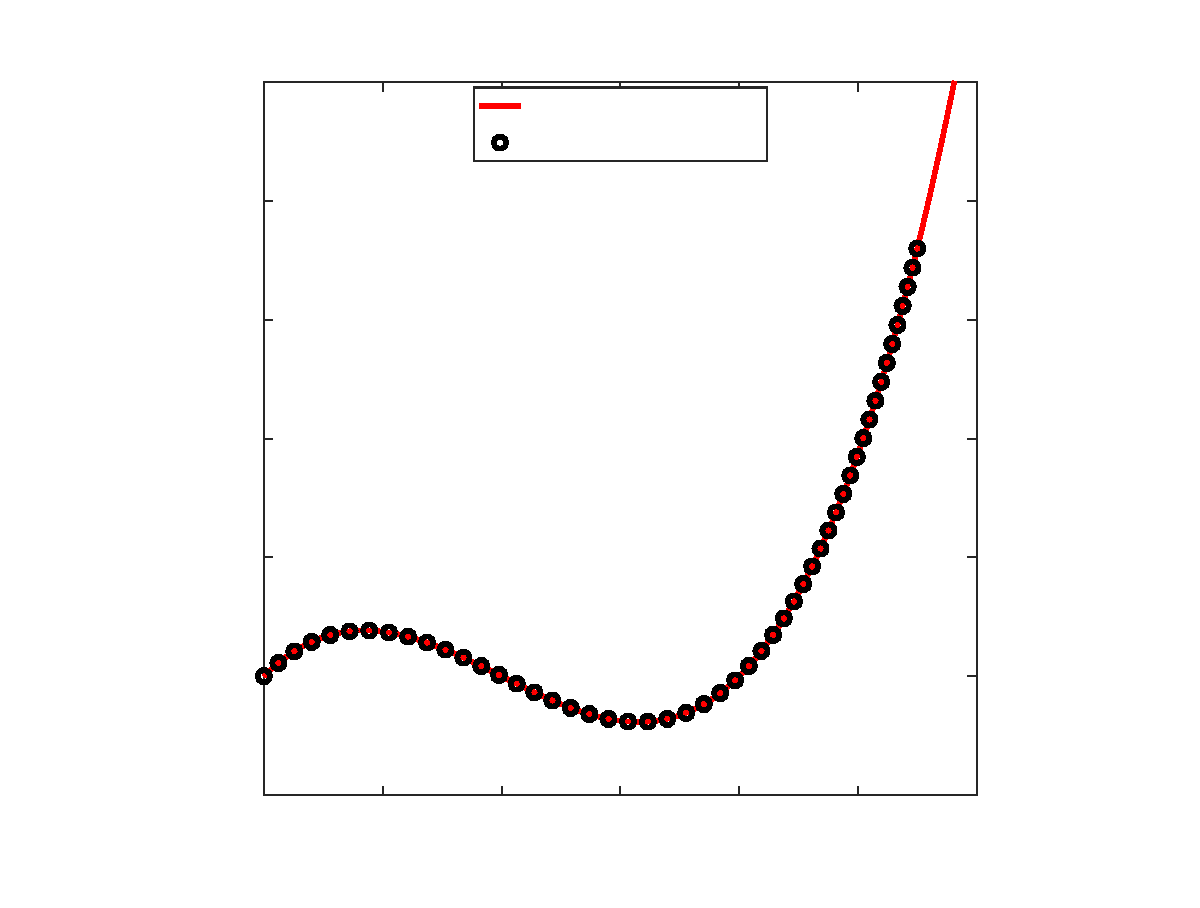
\includegraphics{Fig6Epscargabaja-inc}
\end{picture}%
\begin{picture}(560,420)(0,0)
\fontsize{15}{0}
\selectfont\put(118.65,41.1956){\makebox(0,0)[t]{\textcolor[rgb]{0.15,0.15,0.15}{{0}}}}
\fontsize{15}{0}
\selectfont\put(175.7,41.1956){\makebox(0,0)[t]{\textcolor[rgb]{0.15,0.15,0.15}{{0.5}}}}
\fontsize{15}{0}
\selectfont\put(232.75,41.1956){\makebox(0,0)[t]{\textcolor[rgb]{0.15,0.15,0.15}{{1}}}}
\fontsize{15}{0}
\selectfont\put(289.8,41.1956){\makebox(0,0)[t]{\textcolor[rgb]{0.15,0.15,0.15}{{1.5}}}}
\fontsize{15}{0}
\selectfont\put(346.85,41.1956){\makebox(0,0)[t]{\textcolor[rgb]{0.15,0.15,0.15}{{2}}}}
\fontsize{15}{0}
\selectfont\put(403.9,41.1956){\makebox(0,0)[t]{\textcolor[rgb]{0.15,0.15,0.15}{{2.5}}}}
\fontsize{15}{0}
\selectfont\put(460.95,41.1956){\makebox(0,0)[t]{\textcolor[rgb]{0.15,0.15,0.15}{{3}}}}
\fontsize{15}{0}
\selectfont\put(113.646,46.2){\makebox(0,0)[r]{\textcolor[rgb]{0.15,0.15,0.15}{{-0.5}}}}
\fontsize{15}{0}
\selectfont\put(113.646,103.25){\makebox(0,0)[r]{\textcolor[rgb]{0.15,0.15,0.15}{{0}}}}
\fontsize{15}{0}
\selectfont\put(113.646,160.3){\makebox(0,0)[r]{\textcolor[rgb]{0.15,0.15,0.15}{{0.5}}}}
\fontsize{15}{0}
\selectfont\put(113.646,217.35){\makebox(0,0)[r]{\textcolor[rgb]{0.15,0.15,0.15}{{1}}}}
\fontsize{15}{0}
\selectfont\put(113.646,274.4){\makebox(0,0)[r]{\textcolor[rgb]{0.15,0.15,0.15}{{1.5}}}}
\fontsize{15}{0}
\selectfont\put(113.646,331.45){\makebox(0,0)[r]{\textcolor[rgb]{0.15,0.15,0.15}{{2}}}}
\fontsize{15}{0}
\selectfont\put(113.646,388.5){\makebox(0,0)[r]{\textcolor[rgb]{0.15,0.15,0.15}{{2.5}}}}
\fontsize{14}{0}
\selectfont\put(289.8,23.1956){\makebox(0,0)[t]{\textcolor[rgb]{0.15,0.15,0.15}{{$x$}}}}
\fontsize{14}{0}
\selectfont\put(79.6456,217.35){\rotatebox{90}{\makebox(0,0)[b]{\textcolor[rgb]{0.15,0.15,0.15}{{$\lambda$}}}}}
\fontsize{12}{0}
\selectfont\put(244.634,377){\makebox(0,0)[l]{\textcolor[rgb]{0,0,0}{{Solución Exacta}}}}
\fontsize{12}{0}
\selectfont\put(244.634,359.333){\makebox(0,0)[l]{\textcolor[rgb]{0,0,0}{{Solución Numérica}}}}
\end{picture}
}
	\caption{Soluciones Numéricas con Método de Longitud de Arco.}
	\label{fig:fig6}
\end{figure}

Notar que el método de Longitud de Arco utilizado logra pasar por dos puntos críticos, uno en $x\simeq 0.5$ y otro en $x\simeq 1.5$.

También se puede observar en la Figura \ref{fig:fig6} que los puntos que componen la solución mediante el procedimiento de Longitud de Arco se encuentran equiespaciadas en la longitud de la curva correspondiente a la solución exacta. Se debe notar que para que dichos puntos parezcan equiespaciados, el gráfico debe tener el mismo escalado de ejes que la métrica usada como definición de longitud de arco en la Ecuación~\eqref{ec11}.

El código de Octave utilizado para generar la solución numérica se presenta en el Código~\ref{cod:EjNum3}.

\cajaactividad{
	Estudie cómo cambiar el código dado para poder resolver un sistema de ecuaciones no lineales en $\mathbb{R}^n$.}

%\bigskip

\lstinputlisting[caption = {Solución con Método de Longitud de Arco - Ejemplo Numérico 3.}\label{cod:EjNum3}]{../src/ArcLength1dof.m}







\section{Ejercicios}

%Estas l\'{\i}neas crean el entorno numerado "exercise"
\newcounter{numEjer}[section]
\newenvironment{exercise}[1][]{\addtocounter{numEjer}{1} \noindent \textbf{Ejercicio \arabic{numEjer} #1}}{}




%--------------- EJ1 ----------------------------------------------------------------------

\bigskip
\begin{exercise}
	
	En este ejercicio se usará el Método de Heun como alternativa a Euler Hacia Adelante para calcular una solución puramente Incremental.  El Método de Heun queda definido por:
	%
	\begin{equation*}
		\text{Heun}
		\begin{cases} 
			\bfp_{k+1} = \bfx_k + \Delta \lambda \cdot \bfh(\bfx_k,\lambda_k) \\
			\bfx_{k+1}= \bfx_k + \Delta \lambda \left(\bfh(\bfx_k,\lambda_k) + \bfh(\bfp_{k+1},\lambda_{k+1}) \right)/2\cdot  \\
			\bfx_0=\bfx(0)
		\end{cases}
	\end{equation*}
	
	Se pide:
	\begin{itemize}
		\item[i)] Utilizar el método de Heun para resolver el Ejemplo Numérico 1 con el mismo incremento $\Delta \lambda$ (sugerencia: utilizar el Código~\ref{cod:ejnonlin} como base para su implementación.
		%
		\item[ii)] Comparar la solución de Euler Hacia Adelante con la obtenida en el ítem anterior. Investigue cual es el orden del error cometido por Heun en cada paso y comparar contra el dado presentado para Euler Hacia Adelante.
	\end{itemize}
\end{exercise}

% ------------ EJ2 ---------------------------------------------
\bigskip
\begin{exercise}
	
	Generar mediante el Método de Newton-Raphson tres estimaciones de $\sqrt{2}$ que se expresen como fracciones de números enteros ($\sqrt{2}\simeq p/q$). Realizar el desarrollo y todos los cálculos manualmente.
	
	La primera estimación deberá utilizar enteros de un dígito, la segunda enteros de dos dígitos y la tercera de tres dígitos.
	
	Evaluar los errores absolutos de cada una de las estimaciones y verificar que la convergencia ocurre con orden 2.
	
	\smallskip
	
	\textit{Pregunta Recretiva:} \textquestiondown Existe una mejor aproximación para $\sqrt{2}$ que se exprese como el cociente de dos enteros de dos digitos que la hallada? 
	\bigskip
\end{exercise}


% ------------ EJ2 -------------------------------------------

\begin{exercise}
	
	Resolver el siguiente sistema de ecuaciones no-lineales mediante Newton-Raphson. El sistema de ecuaciones corresponde al ejemplo con dos grados de libertad de la Sección 1.3 de \citep{crisfield1996non}.
	
	$$
	\bff(x)-\lambda \bfv = 0
	$$
	%
	con $\bfx=(x_1,x_2)^T$, $\lambda \in \mathbb{R}^+$, $\bfv=(1,0)^T$
	
	$$\bff(\bfx)= \left(\begin{array}{l}
		- \frac{1}{2} x_2^2 - \epsilon x_2 + x_1 \\
		(\epsilon+x_2)\left(\frac{1}{2}x_2^2+\epsilon x_2 -x_1\right)+x_2 
	\end{array}\right)$$
	
	\bigskip
	
	Resolver para valores: $\epsilon=1/10$, $\epsilon=1/100$ y $\epsilon=1/1000$. 
	
	Dar soluciones para los valores de $\lambda=\{0;0.05;0.10;...;0.95;1.00\}$
	
\end{exercise}



\bigskip
\begin{exercise}

Las siguientes preguntas buscan que se investigue la velocidad y orden de convergencia del método de Newton-Raphson. Asuma en todos los casos que se considera ecuaciones no-lineales de la forma
	$f(x)=0$ con $f:\mathbb{R}\rightarrow \mathbb{R}$.
	\begin{itemize}
		\item[i)] Dar un ejemplo en el cual la iteración de N-R diverge de la raíz buscada.
		
		\item[ii)] Dar un ejemplo en el cual la iteración de N-R se mantiene en un bucle infinito, sin diverger ni converger a la raíz buscada.
		
		\item[iii)] ¿Puede dar un ejemplo en el cual N-R no converge a la raíz buscada con orden 2 sino con orden 1? Verificar numéricamente el orden para el ejemplo propuesto.
	\end{itemize}
	
\end{exercise}


\bigskip
\begin{exercise}
	
	En este ejercicio se plantea trabajar con un método cuasi-Newton y evaluar su orden de convergencia.
	\begin{itemize}
		\item[i)] Resolver el problema presentado en el Ejemplo Numérico 2 utilizando el Método de la Secante.
		
		\item[ii)] Evaluar numéricamente el orden de convergencia del Método de la Secante usando la iteración generada en el item anterior. Compare el valor estimado de orden de convergencia contra el valor teórico dado en las notas del curso.
		
	\end{itemize}
	
\end{exercise}

%%%%%%%%%%%%%%%%%%%%%%%%%%%%%%%%%%%%%%%%%%%%%%%%%%%%%%%%%%%%%


